\documentclass[11pt]{article}

\usepackage[margin=0.75in]{geometry}
\usepackage{amsfonts, amsmath, amssymb}
\usepackage[none]{hyphenat}
\usepackage{fancyhdr}
\usepackage{graphicx}
\usepackage{float}
\usepackage[nottoc, notlot, notlof]{tocbibind}
\usepackage{mathrsfs}
\usepackage{bm}
\usepackage[caption=false]{subfig}




% Packages for code formatting
\usepackage{xcolor}
\usepackage{listings}

% Packages for code formatting
\usepackage{xcolor}
\usepackage{listings}

% Packages for code formatting
\usepackage{xcolor}
\usepackage{listings}

% Define colors
\definecolor{codegreen}{rgb}{0,0.6,0}
\definecolor{codegray}{rgb}{0.5,0.5,0.5}
\definecolor{codepurple}{rgb}{0.58,0,0.82}
\definecolor{backcolour}{rgb}{0.95,0.95,0.92}

% Define Python style for listings with forced line breaking
\lstdefinestyle{pythonstyle}{
    backgroundcolor=\color{backcolour},   
    commentstyle=\color{codegreen},
    keywordstyle=\color{magenta},
    numberstyle=\tiny\color{codegray},
    stringstyle=\color{codepurple},
    basicstyle=\ttfamily\footnotesize,
    breaklines=true,                 % Enable line breaking
    breakatwhitespace=false,         % Allow breaking anywhere
    prebreak=\raisebox{0ex}[0ex][0ex]{\tiny$\hookleftarrow$},  % Show a wrap indicator
    postbreak=\mbox{\textcolor{red}{$\hookrightarrow$}}, % Show continuation symbol
    captionpos=b,                    
    keepspaces=true,                 
    numbers=left,                    
    numbersep=5pt,                  
    showspaces=false,                
    showstringspaces=false,
    showtabs=false,                  
    tabsize=4
}

% Set default style to Python
\lstset{style=pythonstyle}

\pagestyle{fancy}
\fancyhead{}
\fancyfoot{}
\fancyhead[L]{Signals and Systems (course 25742)}
\fancyhead[R]{Reza Nayeb Habib 401102694}
\fancyfoot[C]{\thepage}
\fancyfoot[R]{Sharif University of Technology}
\renewcommand{\footrulewidth}{1pt}
\parindent 0ex

\begin{document}
 
\begin{titlepage}
\begin{center}

\begin{figure}[H]
\begin{center}

\includegraphics[scale=0.4]{Fig/SUT.png}

\end{center}
\end{figure}

\huge{\textbf{Neuroscience of Learning, Memory and Cognition}} \\ 
\vspace*{2cm}
\Large{\textbf{Instructor: Prof. Karbalaei}} \\
\vspace*{1cm}
\huge{\textbf{Sharif University of Technology}} \\
\line(1,0){500} \\ 
\Huge{\textbf{Project: Solving Maze Using Q-Learning Algorithm}} \\
\line(1,0){500} \\
\vfill
\Large{By Reza Nayeb Habib}\\
\Large{Student ID\# 401102694} \\

\end{center}
\end{titlepage}

\tableofcontents
\thispagestyle{empty}
\clearpage
\setcounter{page}{1}


\section{The Maze Generation Algorithm}
The Maze Generation Algorithm is coded as below

\begin{lstlisting}[language=Python]
# Adapted from http://code.activestate.com/recipes/578356-random-maze-generator/
# Random Maze Generator using Depth-first Search
# http://en.wikipedia.org/wiki/Maze_generation_algorithm


import random
import matplotlib.pyplot as plt
import numpy as np

random.seed(401102694)
mx = 20; my = 20 # width and height of the maze

maze = [[0 for x in range(mx)] for y in range(my)]
dx = [0, 1, 0, -1]; dy = [-1, 0, 1, 0] # 4 directions to move in the maze
color = [(0, 0, 0), (255, 255, 255)] # RGB colors of the maze

# start the maze from a random cell
cx = random.randint(0, mx - 1)
cy = random.randint(0, my - 1)
maze[cy][cx] = 1
stack = [(cx, cy, 0)] # stack element: (x, y, direction)

while len(stack) > 0:
    (cx, cy, cd) = stack[-1]
    # to prevent zigzags:
    # if changed direction in the last move then cannot change again
    if len(stack) > 2:
        if cd != stack[-2][2]: dirRange = [cd]
        else: dirRange = range(4)
    else: dirRange = range(4)

    # find a new cell to add
    nlst = [] # list of available neighbors
    for i in dirRange:
        nx = cx + dx[i]
        ny = cy + dy[i]
        if nx >= 0 and nx < mx and ny >= 0 and ny < my:
            if maze[ny][nx] == 0:
                ctr = 0 # of occupied neighbors must be 1
                for j in range(4):
                    ex = nx + dx[j]; ey = ny + dy[j]
                    if ex >= 0 and ex < mx and ey >= 0 and ey < my:
                        if maze[ey][ex] == 1: ctr += 1
                if ctr == 1: nlst.append(i)

    # if 1 or more neighbors available then randomly select one and move
    if len(nlst) > 0:
        ir = nlst[random.randint(0, len(nlst) - 1)]
        cx += dx[ir]; cy += dy[ir]; maze[cy][cx] = 1
        stack.append((cx, cy, ir))
    else: stack.pop()

maze = np.array(maze)
maze -= 1
maze = abs(maze)
        
maze[0][0] = 0
maze[mx-1][my-1] = 0

np.save('maze', np.array(maze))
    
\end{lstlisting}

In the project document it is stated that there is always a path between its
upper left point (0,0) to its lower right point (my-1,mx-1) this statement is
true because the maze Generation Algorithm starts at a random point in the plane
then carves out into different paths by seeing the blocks that have more than 2
wall neighbors (0 in the code) and this algorithm always uses already created path
points neighbors to create new path points thus the maze is always connected. At the
final lines, this algorithm adds (0,0) and (my-1,mx-1) to the path; but how
does it make sure that these two points will be also connected by the previous path? \\
We can ensure these two points are always connected because no cell in this structure
will have more than 2 walls beside it so it means every wall will always have at least
one path neighbor! Thus when for example (0,0) cell is set to 1 it will always have
a neighbor with value one and it will not be an isolated path point and it will be connected
to all other path points.

\section{Drawing The Maze}
The following code draws the Maze by Loading the file and using matplotlib\'s Imshow:


\begin{lstlisting}[language=Python]
maze = np.load('maze.npy')
plt.imshow(1-maze, cmap='gray')   # black is wall white is path
plt.xticks([]); plt.yticks([])
plt.show()
\end{lstlisting}

it gives the following result:
\begin{figure}[H]
    \begin{center}
        
\includegraphics[scale=0.7]{Fig/maze.png}
        \label{fig:xt&xnfft}
        \caption{the unique maze of my student number seed}
    \end{center}
\end{figure}



\section{Q-Learning Algorithm}
\subsection{Full Code and Results}
\begin{lstlisting}[language=Python]
import numpy as np
import random
import matplotlib.pyplot as plt
import imageio
import os

class Environment:
    def __init__(self, maze_file):
        self.maze = np.load(maze_file)
        self.ny, self.nx = self.maze.shape
        self.start = (0, 0)
        self.goal = (self.nx - 1, self.ny - 1)
        self.maze_file = maze_file
        self.output_dir = os.path.join(os.path.dirname(maze_file), "output")
        os.makedirs(self.output_dir, exist_ok=True)  
            # Create output directory if it doesn't exist

    def get_valid_actions(self, x, y):
        """Returns a list of valid actions for a given state."""
        valid_actions = []
        actions = [(0, -1), (1, 0), (0, 1), (-1, 0)]  # Up, Right, Down, Left
        for i, (dx, dy) in enumerate(actions):
            nx_, ny_ = x + dx, y + dy
            if 0 <= nx_ < self.nx and 0 <= ny_ < self.ny and self.maze[ny_][nx_] == 0:
                valid_actions.append(i)
        return valid_actions

    def get_reward(self, x, y):
        """Returns the reward for a given state."""
        if (x, y) == self.goal:
            return 100  # Big reward for reaching the goal
        else:
            return -1  # Small penalty for each step

    def is_goal(self, x, y):
        """Checks if the given state is the goal."""
        return (x, y) == self.goal

    def visualize_maze(self):
        """Visualizes the maze."""
        plt.imshow(self.maze, cmap='gray')
        plt.title("Maze")
        plt.show()

class Agent:
    def __init__(self, env, alpha=0.1, gamma=0.9, epsilon=1.0, 
            epsilon_decay=0.995, epsilon_min=0.01):
        self.env = env
        self.alpha = alpha  # Learning rate
        self.gamma = gamma  # Discount factor
        self.epsilon = epsilon  # Initial exploration rate
        self.epsilon_decay = epsilon_decay  # Decay per episode
        self.epsilon_min = epsilon_min  # Minimum epsilon value
        self.actions = [(0, -1), (1, 0), (0, 1), (-1, 0)]  # Up, Right, Down, Left
        self.num_actions = len(self.actions)
        self.Q_table = np.zeros((env.ny, env.nx, self.num_actions))  # Q-table

    def choose_action(self, x, y):
        """Epsilon-greedy policy."""
        if random.uniform(0, 1) < self.epsilon:
            return random.choice(self.env.get_valid_actions(x, y))  # Explore
        else:
            valid_actions = self.env.get_valid_actions(x, y)
            return max(valid_actions, key=lambda a: self.Q_table[y, x, a])  # Exploit

    def train(self, num_episodes):
        """Trains the agent using Q-learning."""
        for episode in range(num_episodes):
            x, y = self.env.start  # Start position
            total_reward = 0

            while not self.env.is_goal(x, y):  # Until reaching the goal
                action = self.choose_action(x, y)
                dx, dy = self.actions[action]
                new_x, new_y = x + dx, y + dy

                # Reward system
                reward = self.env.get_reward(new_x, new_y)

                # Q-value update
                best_next_action = max(self.env.get_valid_actions(new_x, new_y),
                    key=lambda a: self.Q_table[new_y, new_x, a])
                self.Q_table[y, x, action] += self.alpha * (reward + self.gamma *
                    self.Q_table[new_y, new_x, best_next_action] - self.Q_table[y, x, action])

                x, y = new_x, new_y
                total_reward += reward

            # Decay epsilon
            self.epsilon = max(self.epsilon * self.epsilon_decay, self.epsilon_min)

            if episode % 500 == 0:
                print(f"Episode {episode}, Total Reward: 
                    {total_reward}, Epsilon: {self.epsilon:.3f}")

    def solve_maze(self):
        """Uses the trained Q-table to solve the maze."""
        x, y = self.env.start
        path = [(x, y)]
        while not self.env.is_goal(x, y):
            action = max(self.env.get_valid_actions(x, y),
                key=lambda a: self.Q_table[y, x, a])
            dx, dy = self.actions[action]
            x, y = x + dx, y + dy
            path.append((x, y))
        return path

    def draw_policy(self, episode, save_path=None):
        """Visualizes the best policy at each cell using arrows.
        The optimal path (even if it leads to dead ends) is shown in green.
        """
        fig, ax = plt.subplots(figsize=(10, 10))
        ax.imshow(1 - self.env.maze, cmap="gray")  # Show maze

        arrow_map = {
            0: (0, -1),   # Up
            1: (1, 0),    # Right
            2: (0, 1),    # Down
            3: (-1, 0)    # Left
        }

        # Compute the best current path, even if not optimal (can hit dead ends)
        x, y = self.env.start
        visited = set()
        best_path = []

        while (x, y) not in visited and not self.env.is_goal(x, y):
            visited.add((x, y))
            best_path.append((x, y))

            valid_actions = self.env.get_valid_actions(x, y)
            if not valid_actions:  # If no valid moves, stop
                break
            
            best_action = max(valid_actions, key=lambda a: self.Q_table[y, x, a])
            dx, dy = arrow_map[best_action]
            x, y = x + dx, y + dy

        best_path_set = set(best_path)  # Convert to set for quick lookup

        # Draw policy arrows
        for y in range(self.env.ny):
            for x in range(self.env.nx):
                if self.env.maze[y, x] == 0:  # Ignore walls
                    valid_actions = self.env.get_valid_actions(x, y)
                    if valid_actions:  # If there are valid actions
                        best_action = max(valid_actions, key=lambda a: self.Q_table[y, x, a])
                        dx, dy = arrow_map[best_action]

                        color = 'green' if (x, y) in best_path_set else 'red'
                        ax.arrow(x, y, dx * 0.3, dy * 0.3, head_width=0.2,
                            head_length=0.2, fc=color, ec=color)

        ax.set_title(f"Policy Visualization - Episode {episode}")

        if save_path:
            plt.savefig(save_path)
            plt.close(fig)  # Close the figure to avoid displaying it
        else:
            plt.show()


    def draw_optimal_path(self, path=None, save_path=None):
        """Draws the maze with the optimal path overlaid and optionally saves it as a PNG."""
        if path is None:
            path = self.solve_maze()  # Solve the maze if no path is provided

        fig, ax = plt.subplots(figsize=(10, 10))
        ax.imshow(self.env.maze, cmap="gray")  # Show maze

        # Extract X and Y coordinates from path
        x_coords, y_coords = zip(*path)

        # Plot the path with red line
        ax.plot(x_coords, y_coords, color='red', linewidth=2, marker='o'
            , markersize=4, label="Optimal Path")

        # Mark start and goal positions
        ax.scatter([self.env.start[0]], [self.env.start[1]], color='green'
            , s=100, label="Start (0,0)")
        ax.scatter([self.env.goal[0]], [self.env.goal[1]], color='blue'
            , s=100, label=f"Goal ({self.env.goal[0]},{self.env.goal[1]})")

        ax.legend()
        plt.title("Optimal Path in the Maze")

        if save_path:
            plt.savefig(save_path)
            plt.close(fig)  # Close the figure to avoid displaying it
        else:
            plt.show()

    def train_with_visualization(self, num_episodes, frame_time, d_episode):
        """Trains the agent and saves a GIF of the policy evolution."""
        frames = []  # List to store frames

        for episode in range(num_episodes):
            x, y = self.env.start  # Start position
            total_reward = 0

            while not self.env.is_goal(x, y):  # Until reaching the goal
                action = self.choose_action(x, y)
                dx, dy = self.actions[action]
                new_x, new_y = x + dx, y + dy

                # Reward system
                reward = self.env.get_reward(new_x, new_y)

                # Q-value update
                best_next_action = max(self.env.get_valid_actions(new_x, new_y), 
                    key=lambda a: self.Q_table[new_y, new_x, a])
                self.Q_table[y, x, action] += self.alpha * (reward + self.gamma * 
                    self.Q_table[new_y, new_x, best_next_action] - self.Q_table[y, x, action])

                x, y = new_x, new_y
                total_reward += reward

            # Decay epsilon
            self.epsilon = max(self.epsilon * self.epsilon_decay, self.epsilon_min)

            # Save policy visualization at key episodes
            if episode % d_episode == 0 or episode == num_episodes - 1:
                save_path = os.path.join(self.env.output_dir, f"policy_episode_{episode}.png")
                self.draw_policy(episode, save_path)
                frames.append(imageio.imread(save_path))  # Store frame

            if episode % d_episode == 0:
                print(f"Episode {episode}, Total Reward: {total_reward},
                    Epsilon: {self.epsilon:.3f}")

        # Save GIF with longer duration between frames
        gif_path = os.path.join(self.env.output_dir, "policy_evolution.gif")
        imageio.mimsave(gif_path, frames, duration=frame_time*num_episodes/d_episode)
        print(f"GIF saved as {gif_path}")

        # Clean up temporary files
        for episode in range(0, num_episodes, d_episode):
            os.remove(os.path.join(self.env.output_dir, f"policy_episode_{episode}.png"))
        os.remove(os.path.join(self.env.output_dir, f"policy_episode_{num_episodes - 1}.png"))


# Main execution
if __name__ == "__main__":
    env = Environment('.\\maze.npy')
    agent = Agent(env)

    # Train the agent
    agent.train_with_visualization(num_episodes=1000, frame_time=5.0, d_episode=25)

    # Solve the maze and visualize the optimal path
    solution_path = agent.solve_maze()
    
    optimal_path_image_path = os.path.join(env.output_dir, "optimal_path.png")
    
    agent.draw_optimal_path(solution_path, save_path=optimal_path_image_path)
    print(f"Optimal path visualization saved as {optimal_path_image_path}")
    agent.draw_optimal_path(solution_path)
\end{lstlisting}

This code gives the following Results (the Gif file is included in the zip sent with this pdf file):
\begin{figure}[H]
    \begin{center}
        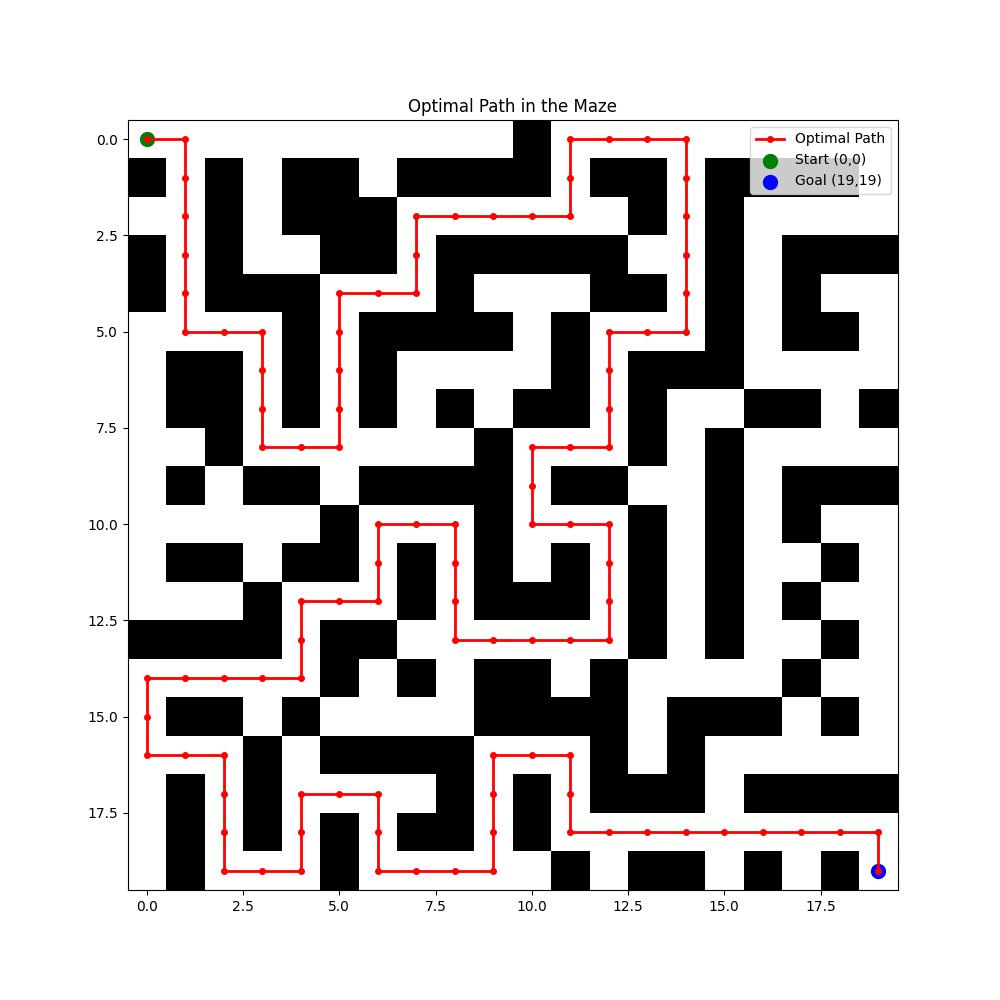
\includegraphics[scale=0.55]{Fig/optimal_path.png}
        \label{fig:optimalPath}
        \caption{the Optimal path in the maze found by Q-learning}
    \end{center}
\end{figure}

\begin{figure}[H]
    \begin{center}
        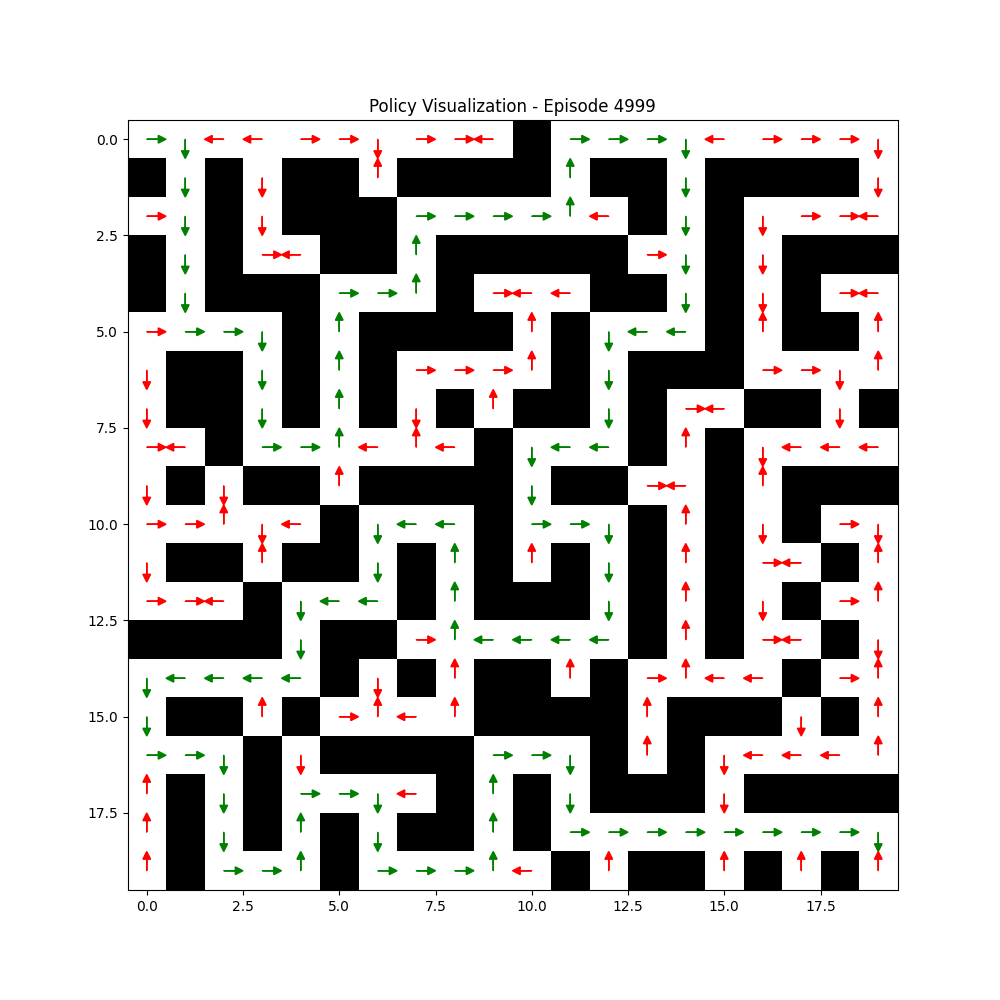
\includegraphics[scale=0.55]{Fig/optimal_policy.png}
        \label{fig:optimalPath}
        \caption{the Optimal policy in the maze found by Q-learning}
    \end{center}
\end{figure}

\subsection{Code Explanation}

\texttt{Environment}: \\
This class contains the maze cells mapping the reward function of the maze and the path
the maze file is loaded from. It\'s variables contain the goal point of the maze, the start point of the maze,
the maze shape and ... \\

\texttt{get\_valid\_action(x,y)}: \\
This method of the \texttt{Environment} class gives the valid actions that can be taken
at position (x,y) without hitting a wall or going outside of the maze.

\texttt{get\_reward(x,y)}: \\
This method gives the reward of any given cell (x,y). all cells have a default reward of -1
to avoid the agent from wandering and punish him for taking longer paths. Also the goal point has a reward
of 100 for motivating the agent to reach the end point.

\texttt{is\_goal(x,y)}: \\
Checks if the cell is the goal cell; useful in functions needing to check if they have
reached the end of the maze or not. Returns True if (nx,ny) is given.
\\ \\ 
\texttt{visualize\_maze()}: \\
Uses \texttt{Imshow} to draw the maze.
\\ \\
\texttt{Agent}: \\
This class creates an agent that uses Q-Learning (Explained Later) to find the best
policy for traversing in the maze. This class has the Environment, learning rate, Discount Factor,
exploration rate and its decay factor, and the Q-table as its variables. It creates Q-table from
the size of the maze and the number of actions that can be taken (number of directions that can be traversed)
and Initializes them as zeros.
\\ \\
\texttt{choose\_action(x,y)}: \\
This method of the Agent class is essentially the actor in actor-critic algorithm.
It uses the Q-table to choose the best policy and act on that policy, this action is called exploitation;
It also does exploration by generating a random value between 0 and 1 and if the value is smaller
than the exploration probability (epsilon) it chooses its action randomly from valid actions.
\\ \\
\texttt{train(num\_episodes)} and \texttt{train\_with\_visualization(num\_episodes, frame\_time, d\_episode)}: \\
These functions implement the formula for Q-learning as stated below:
\begin{equation}
    Q(s, a) \leftarrow Q(s, a) + \alpha \left[ r + \gamma \max_{a'} Q(s', a') - Q(s, a) \right]
\end{equation}

by this line of code:
\begin{lstlisting}[language=Python]
    self.Q_table[y, x, action] += self.alpha * (reward + self.gamma 
        * self.Q_table[new_y, new_x, best_next_action] - self.Q_table[y, x, action])
\end{lstlisting}
In every iteration it chooses an action by \texttt{choose\_action(x,y)} and then updates the Q-table
according the action taken. This process is repeated until the goal state is reached, then the episode is done
and a new one starts it iterates this until the number of given episodes of learning is reached. The function with
visualize is the same it only Visualizes the best policy using \texttt{draw\_policy()} and saves it periodically
on specific period of episodes; after that it creates a gif from the given files and saves it in the output folder.
\\ \\
\texttt{draw\_policy(episode, save\_path=None)} \\
This function first draws the maze with \texttt{Imshow} then uses \texttt{scatter} to draw the
best policy at each cell with an arrow (it draws the arrows on the optimal path with green and others with red).
\\ \\
\texttt{draw\_optimal\_path (path=None, save\_path =None):} \\
This function finds the optimal path by using \texttt{solve\_maze()} and getting the path
that will be taken on exploitation mode and again uses scatter for drawing the optimal path given by \texttt{solve\_maze}.
\\ \\
\texttt{solve\_maze()}: \\
This fucntion follows the path given by Q-table until it reaches the goal point. It should
not be used before the model is completely trained to reach the goal point otherwise it will enter
an infinite loop.


\subsection{Deep Q-Learning Implementation}
The Deep Q-Learning algorithm is very similar to normal Q-Learning. The difference is that
the state variables (here x and y) are fed into a deep neural network and it gives the Q value for all
possible actions. Here we show how we implemented this with pytorch: \\

\begin{lstlisting}[language=Python]
import numpy as np
import random
import torch
import torch.nn as nn
import torch.optim as optim
import torch.nn.functional as F
import matplotlib.pyplot as plt
import imageio
import os
from collections import deque

# Environment Class
class Environment:
    def __init__(self, maze_file):
        self.maze = np.load(maze_file)
        self.ny, self.nx = self.maze.shape
        self.start = (0, 0)
        self.goal = (self.nx - 1, self.ny - 1)
        self.actions = [(0, -1), (1, 0), (0, 1), (-1, 0)]  # Up, Right, Down, Left
        self.output_dir = os.path.join(os.path.dirname(maze_file), "output_dqn")
        os.makedirs(self.output_dir, exist_ok=True)

    def get_valid_actions(self, x, y):
        """Returns a list of valid actions for a given state."""
        valid_actions = []
        for i, (dx, dy) in enumerate(self.actions):
            nx_, ny_ = x + dx, y + dy
            if 0 <= nx_ < self.nx and 0 <= ny_ < self.ny and self.maze[ny_, nx_] == 0:
                valid_actions.append(i)
        return valid_actions

    def get_reward(self, x, y):
        """Returns the reward for a given state."""
        return 100 if (x, y) == self.goal else -1

    def is_goal(self, x, y):
        """Checks if the given state is the goal."""
        return (x, y) == self.goal

# Deep Q-Network (DQN) Model
class DQN(nn.Module):
    def __init__(self, input_dim, output_dim):
        super(DQN, self).__init__()
        self.fc1 = nn.Linear(input_dim, 128)
        self.fc2 = nn.Linear(128, 128)
        self.fc3 = nn.Linear(128, output_dim)

    def forward(self, x):
        x = F.relu(self.fc1(x))
        x = F.relu(self.fc2(x))
        return self.fc3(x)

# DQN Agent
class DQNAgent:
    def __init__(self, env, gamma=0.9, lr=0.001, batch_size=64, memory_size=50000):
        self.env = env
        self.gamma = gamma
        self.batch_size = batch_size
        self.epsilon = 1.0
        self.epsilon_decay = 0.995
        self.epsilon_min = 0.01
        self.memory = deque(maxlen=memory_size)

        self.model = DQN(2, len(env.actions))
        self.target_model = DQN(2, len(env.actions))
        self.target_model.load_state_dict(self.model.state_dict())
        self.optimizer = optim.Adam(self.model.parameters(), lr=lr)

    def get_state(self, x, y):
        """Encodes state as a tensor."""
        return torch.tensor([x / self.env.nx, y / self.env.ny], dtype=torch.float32)

    def choose_action(self, x, y):
        """Epsilon-greedy policy."""
        if random.random() < self.epsilon:
            return random.choice(self.env.get_valid_actions(x, y))
        else:
            state = self.get_state(x, y).unsqueeze(0)
            q_values = self.model(state)
            valid_actions = self.env.get_valid_actions(x, y)
            return max(valid_actions, key=lambda a: q_values[0, a].item())

    def store_experience(self, state, action, reward, next_state, done):
        """Stores experience in replay memory."""
        self.memory.append((state, action, reward, next_state, done))

    def train(self):
        """Trains the model using replay memory."""
        if len(self.memory) < self.batch_size:
            return

        batch = random.sample(self.memory, self.batch_size)
        states, actions, rewards, next_states, dones = zip(*batch)

        states = torch.stack(states)
        next_states = torch.stack(next_states)
        actions = torch.tensor(actions, dtype=torch.long)
        rewards = torch.tensor(rewards, dtype=torch.float32)
        dones = torch.tensor(dones, dtype=torch.float32)

        q_values = self.model(states).gather(1, actions.unsqueeze(1)).squeeze(1)
        next_q_values = self.target_model(next_states).max(1)[0].detach()
        target_q_values = rewards + self.gamma * next_q_values * (1 - dones)

        loss = F.mse_loss(q_values, target_q_values)
        self.optimizer.zero_grad()
        loss.backward()
        self.optimizer.step()

    def update_target_network(self):
        """Updates target network weights."""
        self.target_model.load_state_dict(self.model.state_dict())

    def train_agent(self, num_episodes, update_target_every=50, frame_time=5.0, d_episode=50):
        """Trains the DQN agent and creates a GIF."""
        frames = []
        for episode in range(num_episodes):
            x, y = self.env.start
            total_reward = 0
            state = self.get_state(x, y)

            while not self.env.is_goal(x, y):
                action = self.choose_action(x, y)
                dx, dy = self.env.actions[action]
                new_x, new_y = x + dx, y + dy

                reward = self.env.get_reward(new_x, new_y)
                next_state = self.get_state(new_x, new_y)
                done = self.env.is_goal(new_x, new_y)

                self.store_experience(state, action, reward, next_state, done)
                self.train()

                x, y = new_x, new_y
                state = next_state
                total_reward += reward

            self.epsilon = max(self.epsilon * self.epsilon_decay, self.epsilon_min)

            if episode % update_target_every == 0:
                self.update_target_network()

            if episode % d_episode == 0:
                save_path = os.path.join(self.env.output_dir, f"policy_{episode}.png")
                self.visualize_policy(save_path)
                frames.append(imageio.imread(save_path))

            print(f"Episode {episode}, Total Reward: {total_reward}, Epsilon: {self.epsilon:.3f}")

        gif_path = os.path.join(self.env.output_dir, "policy_evolution.gif")
        imageio.mimsave(gif_path, frames, duration=frame_time*num_episodes/d_episode)
        print(f"GIF saved as {gif_path}")

    def visualize_policy(self, save_path=None):
        """Visualizes the current policy."""
        fig, ax = plt.subplots(figsize=(10, 10))
        ax.imshow(1 - self.env.maze, cmap="gray")

        for y in range(self.env.ny):
            for x in range(self.env.nx):
                if self.env.maze[y, x] == 0:
                    best_action = max(self.env.get_valid_actions(x, y), key=lambda a: self.model(self.get_state(x, y).unsqueeze(0))[0, a].item())
                    dx, dy = self.env.actions[best_action]
                    ax.arrow(x, y, dx * 0.3, dy * 0.3, head_width=0.2, head_length=0.2, fc="red", ec="red")

        if save_path:
            plt.savefig(save_path)
            plt.close()
        else:
            plt.show()

# Main Execution
if __name__ == "__main__":
    env = Environment("maze100.npy")
    agent = DQNAgent(env)
    agent.train_agent(num_episodes=5000)

    # Save final policy visualization
    final_policy_path = os.path.join(env.output_dir, "final_policy.png")
    agent.visualize_policy(final_policy_path)

\end{lstlisting}
\end{document}